\section{Análisis y comparación de los algoritmos}

% Marty y el Doc son amigos de nuevo, pero les genera muchas dudas el no tener
% una garantía teórica de optimalidad. Para lo cual les piden, si fueran tan
% amables, que una vez elegidos los mejores valores de configuración para cada
% heurística implementada (si fue posible), realicen una experimentación sobre
% un conjunto nuevo de instancias para observar la performance de los métodos,
% comparando nuevamente la calidad de las soluciones obtenidas y los tiempos
% de ejecución en función del tamaño de entrada. Para los casos en los que sea
% posible, les encantaría comparar también los resultados contra los del
% algoritmo exacto. Ambos personajes son muy exigentes en cuanto a la
% representación de la información y la evidencia científica, con lo cual
% deben presentarles todos los resultados obtenidos mediante gráficos
% adecuados (u otras opciones que consideren provechosas) y discutir al
% respecto de los mismos.

Para concluir el trabajo, se pedía comparar las heurísticas anteriores con
un conjunto de instancias nuevo. Para esto se decidió construir una familia
de instancias para las que fuera posible conocer el resultado exacto, aun
sin necesidad de correr el algoritmo. A continuación se presenta dicha
familia, y se muestra cuál es la solución correcta del problema de \acr{MCS}
para la misma.

\begin{itemize}
    \item $G_1$ es un camino simple con $r$ nodos, es decir, $G_1 = P_r$.
    \item $G_2$ es un bipartito completo con particiones de $s$ y $t$ nodos,
    es decir, $G_2 = K_{s,t}$, con $s < t$.
    \item Además, se cumple que $r \geq t$.
\end{itemize}

En tal caso, la solución de \acr{MCS}, por ser isomorfa a un subgrafo de
$G_1$, deberá ser un camino simple o una unión de caminos simples. En otras
palabras, deberemos buscar caminos simples que sean subgrafos de $G_1$. Ahora
bien, por ser $G_1$ bipartito, todo camino simple dentro del mismo deberá
alternar un nodo de cada partición. Como la menor de las particiones tiene $s$
nodos, es claro que no puede haber ningún camino con más de $2s + 1$ nodos que
sea subgrafo de $G_2$. Más aún, tal camino existe: si se toma de forma
sucesiva un nodo de cada partición, comenzando por la que tiene $t$ nodos, dos
nodos consecutivos siempre estarán unidos por una arista, por ser $G_2$
bipartito completo. Este proceso termina cuando se acaban los nodos de la
partición más chica, es decir, al haber tomado $s$ nodos de cada partición;
entonces, todavía es posible extender el camino con un último nodo de la otra
partición (por ser $t > s$), pero ya no se podrá conectar este último a un
nodo de $s$.

De lo anterior, deducimos que existe un subgrafo de $G_2$ isomorfo a
$P_{2s+1}$. Claramente, $P_{2s+1}$ también es isomorfo a un subgrafo de $G_1$.
Por otra parte, la cantidad de aristas de este grafo es máxima entre los de
este tipo: cualquier otra arista que se intente agregar y que sea respetada en
$G_2$ por el isomorfismo unirá un nodo de cada partición de este grafo, es
decir, y todos los nodos de la partición más chica ya están mapeados por el
isomorfismo a algún nodo de $G_1$, donde sus dos aristas ya están mapeadas a
otras aristas de $G_2$.

En conclusión, el \acr{MCS} entre $G_1$ y $G_2$ es $P_{2s+1}$, que tiene
exactamente $2s$ aristas; este valor puede ser utilizado como parámetro para
medir de forma precisa la calidad de las soluciones brindadas por cada
una de las heurísticas implementadas.

\begin{center}

\begin{tabular}{c|c|c}
Heurística                             & Cant. de aristas encontradas & Porcentaje de la sol. exacta \\ \hline
Solución exacta                        &                              &                              \\
Heurística golosa (G)                  &                              &                              \\
Búsqueda local (Vecindad I) (LS1)      &                              &                              \\
Búsqueda local (Vecindad II) (LS2)     &                              &                              \\
\emph{Tabu search} (Vecindad I) (TS2)  &                              &                              \\
\emph{Tabu search} (Vecindad II) (TS2) &                              &                              \\
\end{tabular}

\end{center}

\begin{figure}[H]
    \centering
    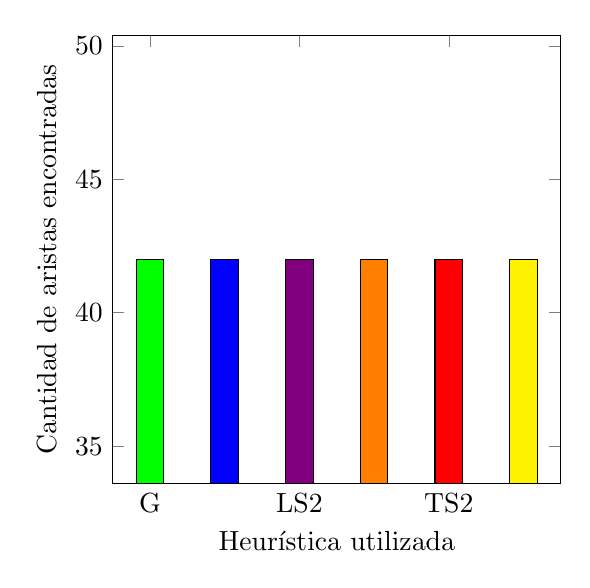
\begin{tikzpicture}[baseline]
        \begin{axis}[
                title={},
                xlabel={Heurística utilizada},
                ylabel={Cantidad de aristas encontradas},
                scaled x ticks=false,
                scaled y ticks=false,
                width=0.6\textwidth,
                height=0.6\textwidth,
                legend pos=outer north east,
                legend cell align=left,
                symbolic x coords={G,LS1,LS2,TS1,TS2,MCS},
            ]
            xtick=data]
            \addplot[ybar,fill=green] coordinates {(G,42)};
            \addplot[ybar,fill=blue] coordinates {(LS1,42)};
            \addplot[ybar,fill=violet] coordinates {(LS2,42)};
            \addplot[ybar,fill=orange] coordinates {(TS1,42)};
            \addplot[ybar,fill=red] coordinates {(TS2,42)};
            \addplot[ybar,fill=yellow] coordinates {(MCS,42)};
        \end{axis}
    \end{tikzpicture}
\end{figure}
